\documentclass[
	ngerman,
	aspectratio=43,
	color={accentcolor=11c},
	logo=false,
	colorframetitle=false,
	]{tudabeamer}
\usepackage[main=ngerman]{babel}
\usepackage{movie15}
\usepackage{tikz}
\usepackage{xcolor}
\usepackage{ulem}
\usepackage{lipsum}

\makeatletter
    \newenvironment{image-frame}{
    	\setbeamertemplate{beamercolorbox}{}
    	\setbeamercolor{background canvas}{bg=black}
        \setbeamertemplate{frametitle}[default]
        \setbeamertemplate{headline}[default]
        \setbeamertemplate{footline}[default]{}
        \def\beamer@entrycode{\vspace*{-\headheight}}
    }{}
\makeatother

\newcommand\blfootnote[1]{%
  \begingroup
  \renewcommand\thefootnote{}\footnote{#1}%
  \addtocounter{footnote}{-1}%
  \endgroup
}

\let\footnoterule\relax
\let\code\texttt

\title{Seminar Algorithmen zum Fahrplanentwurf}
\subtitle{Graphenmodelle}
\author[R. Buhlmann]{Robin Buhlmann}
\department{Fachgebiet Algorithmik}

%\logo*{\includegraphics{example-image-16x9}}
\titlegraphic*{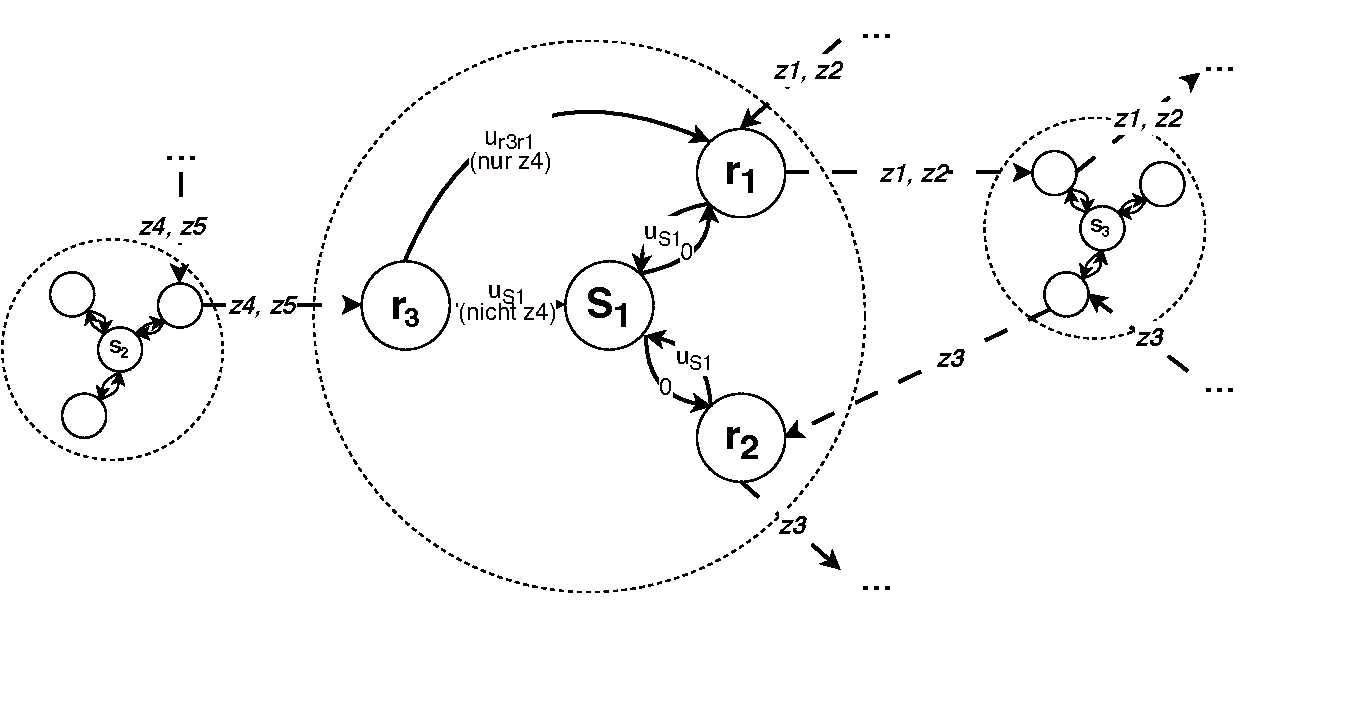
\includegraphics[width=.52\linewidth]{images/main.pdf}}
\date{20.01.2024}

%\AtBeginSection[]
%{
%  \begin{frame}{Übersicht}
%    \tableofcontents[currentsection]
%  \end{frame}
%}

\begin{document}

%\footnotesize{8pt}
\maketitle

\begin{frame}{Analoge Fahrpläne}
\framesubtitle{Wie man sie kennt und nie benutzt...}
	\begin{center}
		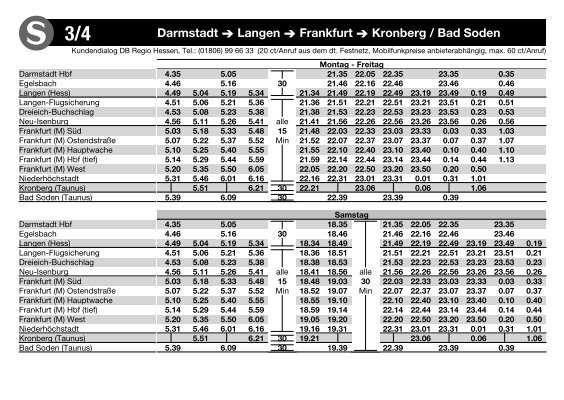
\includegraphics[width=.8\linewidth]{images/fahrplan-s3s4.jpg}
	\end{center}
\end{frame}

\begin{frame}{Fahrplanauskunftssysteme}
	\vspace{4em}
	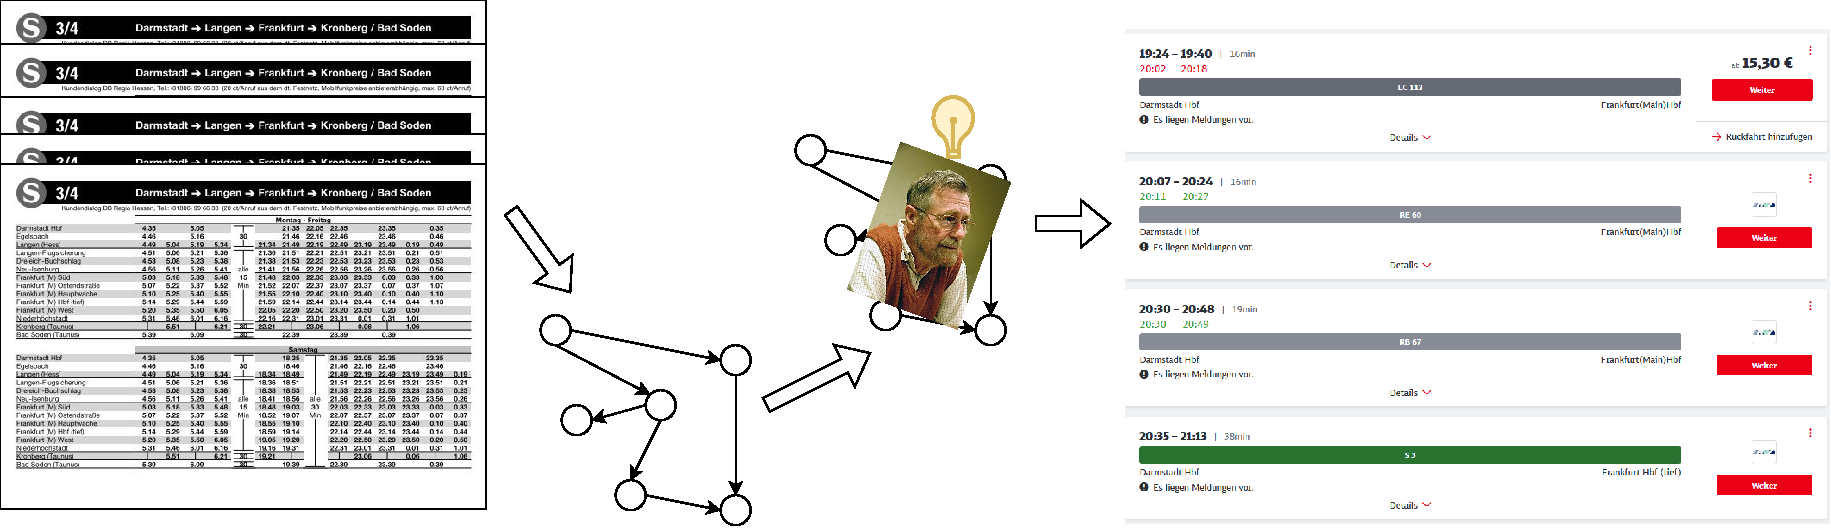
\includegraphics[width=\linewidth]{images/fahrplan-zu-auskunftssystem.pdf}
\end{frame}

\begin{frame}{Fahrplanauskunftssysteme}
	\vspace{3em}
	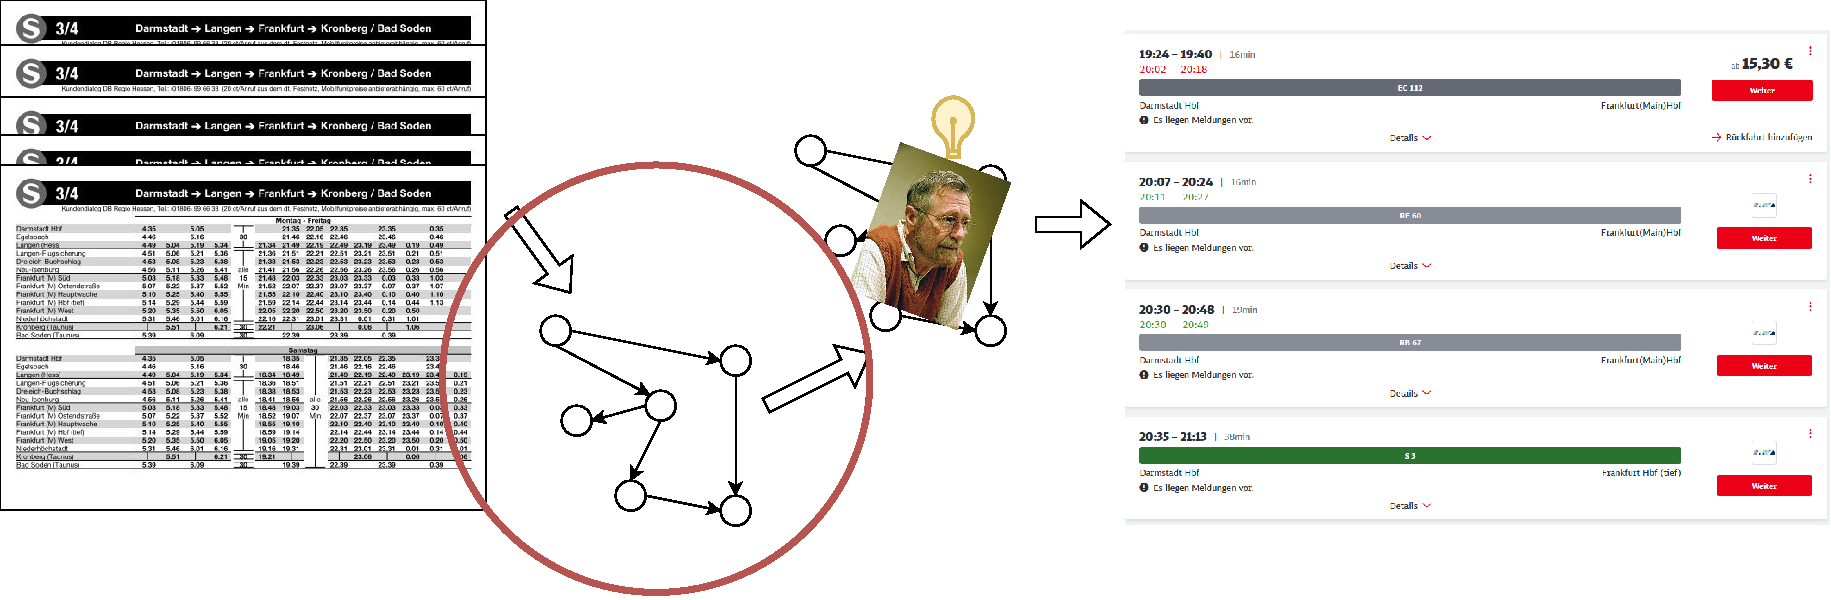
\includegraphics[width=\linewidth]{images/fahrplan-zu-auskunftssystem-2.pdf}
\end{frame}


\begin{frame}{Frage 1}
	\vspace{7em}
	\begin{center}
		\begin{Large}
			Wie wandle ich Fahrpläne zu Graphen um?
		\end{Large}
	\end{center}
\end{frame}

\begin{frame}{Frage 2}
	\vspace{6em}
	\begin{center}
		\begin{Large}
			Wie modelliere ich meinen Graphen, um das Earliest-Arrival Problem zu lösen?
		\end{Large}
	\end{center}
\end{frame}


\begin{frame}{Überblick}
	\begin{itemize}
		\item Grundlagen
	\end{itemize}
	\vspace{1em}
	\begin{itemize}
		\item Das 1. Graphenmodell
		\begin{itemize}
			\item Verfeinerungen
		\end{itemize}
	\end{itemize}
	\vspace{1em}
	\begin{itemize}
		\item Das 2. Graphenmodell
		\begin{itemize}
			\item Verfeinerungen
		\end{itemize}
	\end{itemize}
	\vspace{1em}
	\begin{itemize}
		\item Vergleiche
	\end{itemize}
	\vspace{1em}
	\begin{itemize}
		\item Zusammenfassung
	\end{itemize}
\end{frame}


\section{Terminologie}
\begin{frame}{1. Griff in die Terminologie-Kiste}
	\framesubtitle{Züge und Stationen}

	\begin{block}{}
		Was ist ein Zug?
	\end{block}
	
	\begin{center}
		\begin{tikzpicture}
			\node (img1) {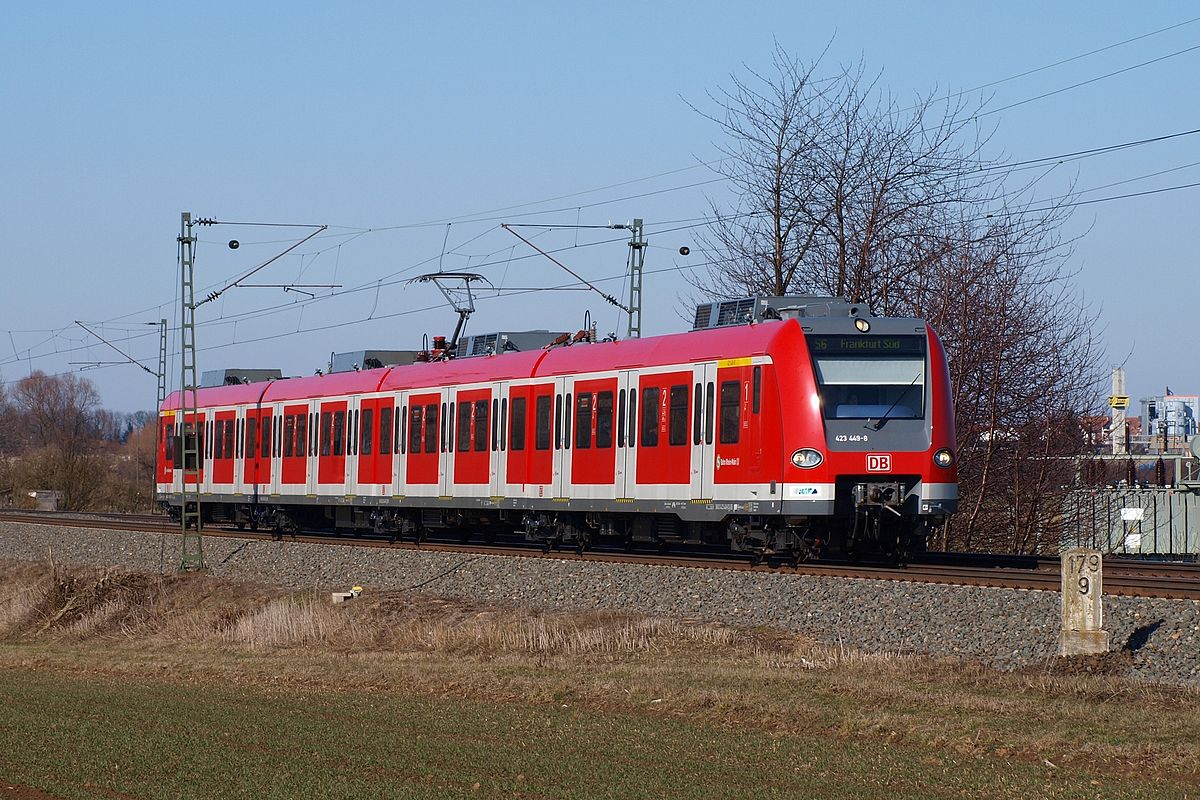
\includegraphics[height=4.5cm]{images/sbahn.jpg}};
			\pause
			\node (img2) at (img1.center) {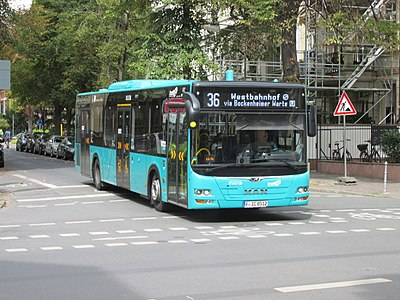
\includegraphics[height=4.5cm]{images/bus.jpg}};
			\pause
			\node (img3) at (img2.center) {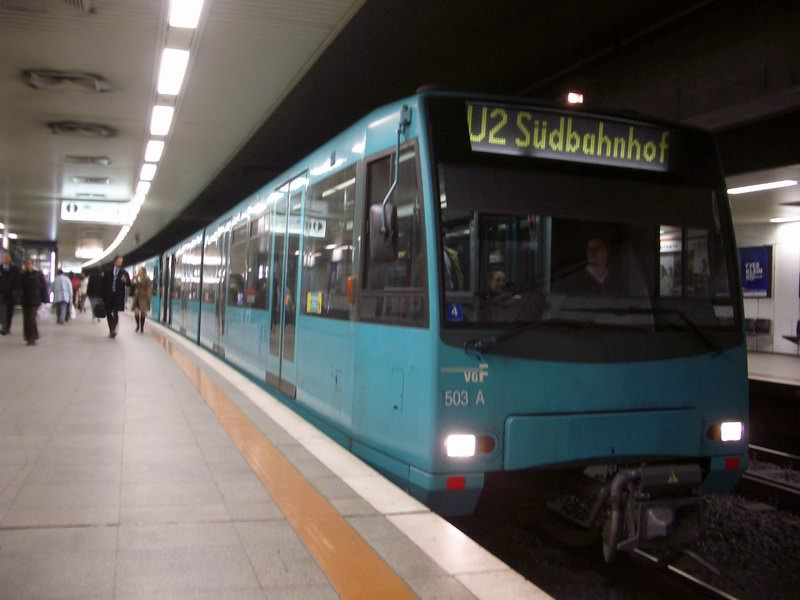
\includegraphics[height=4.5cm]{images/ubahn.jpg}};
			\pause
			\node (img4) at (img3.center) {\includegraphics[height=4.5cm]{images/fähre.jpg}};
		\end{tikzpicture}
	\end{center}
\end{frame}

\begin{frame}{1. Griff in die Terminologie-Kiste}
	\framesubtitle{Züge und Stationen}

	\begin{block}{}
		Was ist eine Station?
	\end{block}
	
	\begin{center}
		\begin{tikzpicture}
			\node (img1) {\includegraphics[height=4.5cm]{images/köppern.jpg}};
			\pause
			\node (img2) at (img1.center) {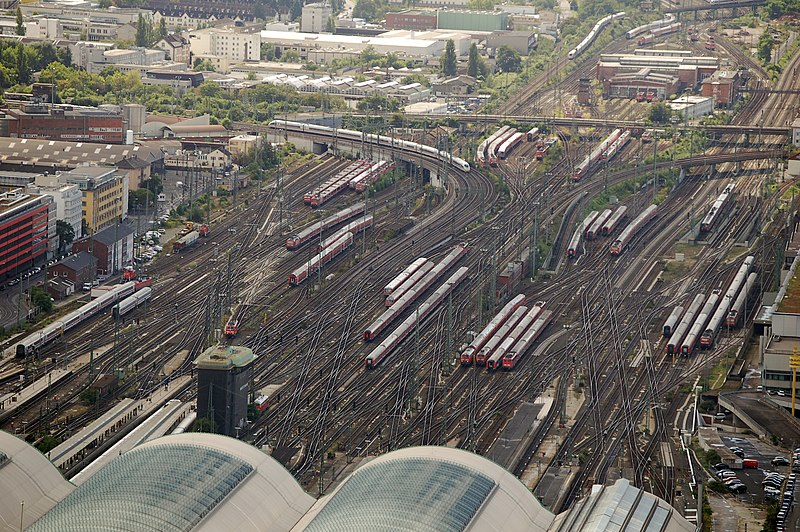
\includegraphics[height=4.5cm]{images/ffm.jpg}};
		\end{tikzpicture}
	\end{center}
\end{frame}


\begin{frame}{Größenordnungen}
	\begin{itemize}
		\item Ein paar Zahlen im Jahr 2008 (\textbf{nur} Züge):
	\end{itemize}

	\vspace{3em}
	\begin{center}
		\begin{tabular}{ c|c } 
			Anzahl & \\
 			\hline
 			Stationen & etwa\texttrademark{} 5000 \\
 			Züge & 68073 \\ 
 			Fußwege & 425 \\
		\end{tabular}
	\end{center}
\end{frame}


\subsection{Naive Ansätze}
\begin{frame}{Wie modelliere ich einen Fahrplan als Graphen?}
	\begin{itemize}
		\item Simple Idee: Knoten sind Stationen, Kanten sind Verbindungen 
	\end{itemize}
	
	\vspace{3em}
	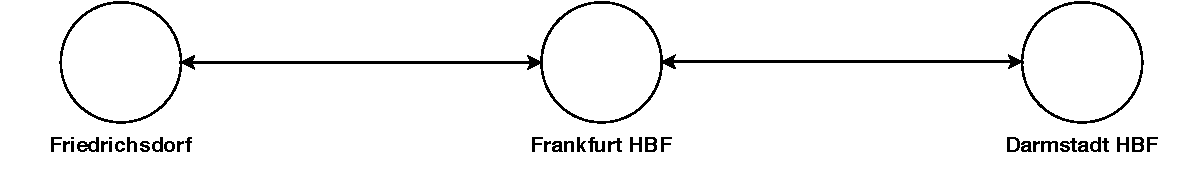
\includegraphics[width=\linewidth]{images/simple-approach.pdf}
	\vspace{3em}
	\begin{block}{}
		Was ist das Problem hier?
	\end{block}
\end{frame}

\begin{frame}{Wie modelliere ich einen Fahrplan als Graphen?}
	\begin{itemize}
		\item Wir müssen irgendwie Zeitverhältnisse innerhalb des Graphen darstellen!
	\end{itemize}
	
	\begin{center}
		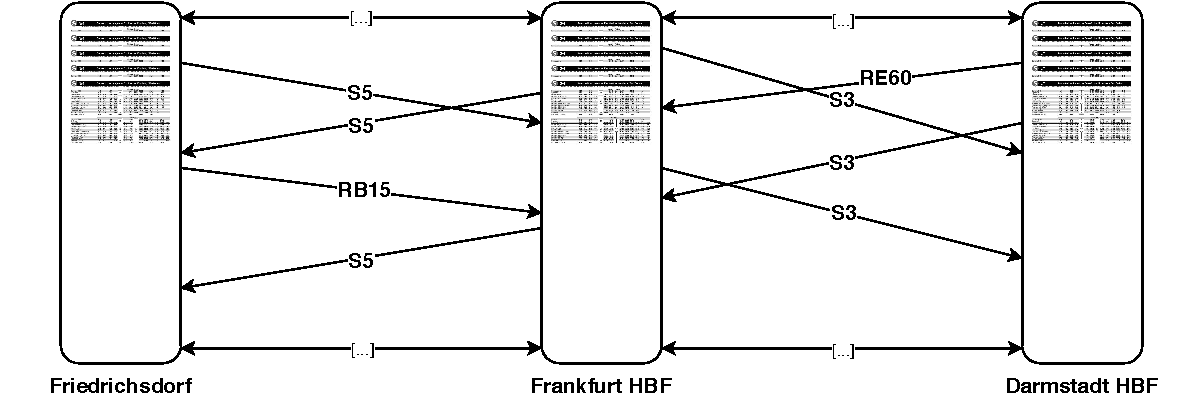
\includegraphics[width=\linewidth]{images/simple-approach-timed.pdf}
	\end{center}

	\begin{block}{}
		Was ist das Problem hier?
	\end{block}
\end{frame}

%\begin{frame}
%	\begin{itemize}
%		\item Wir müssen irgendwie Zeitverhältnisse innerhalb des Graphen darstellen!
%	\end{itemize}
%	
%	\begin{center}
%		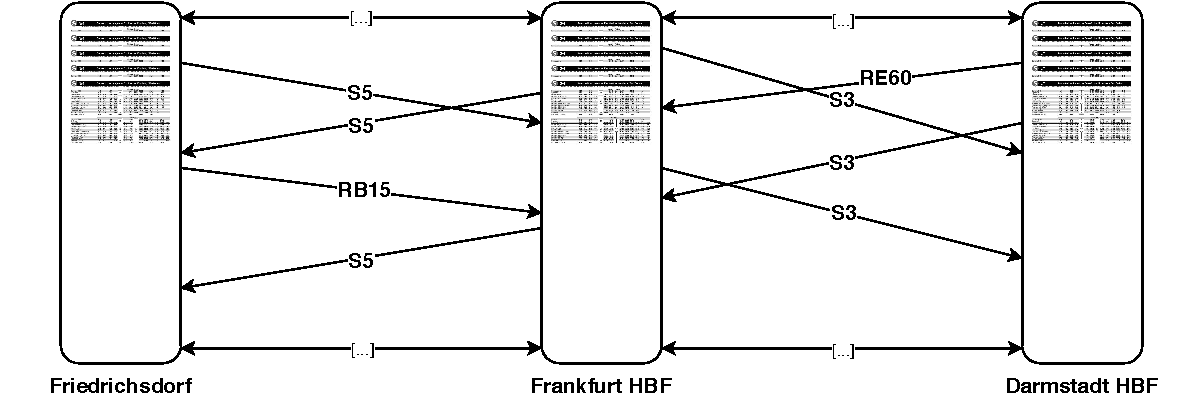
\includegraphics[width=\linewidth]{images/simple-approach-timed-2.pdf}
%	\end{center}
%
%	\begin{block}{}
%		Was ist das Problem hier?
%	\end{block}
%\end{frame}

\begin{frame}{Probleme}
	\framesubtitle{Die es zu lösen gilt...}
	\begin{itemize}
		\item Zeitverhältnisse im Graphen \pause
		\item \textbf{Takt}fahrpläne \pause
		\item Umstiege bzw. Umsteigezeiten \pause		
		\item Fußwege zwischen / innerhalb von Stationen \pause
		\item \sout{Intermodalität}
	\end{itemize}
	
	\vspace{6em}
	\begin{block}{Zwei gängige Modelle}
		Time-Expanded vs. Time-Dependent
	\end{block}
\end{frame}






















\section{Modell 1: Time-Expanded}
%\begin{frame}
%	\vspace{2em}
%	\begin{center}
%		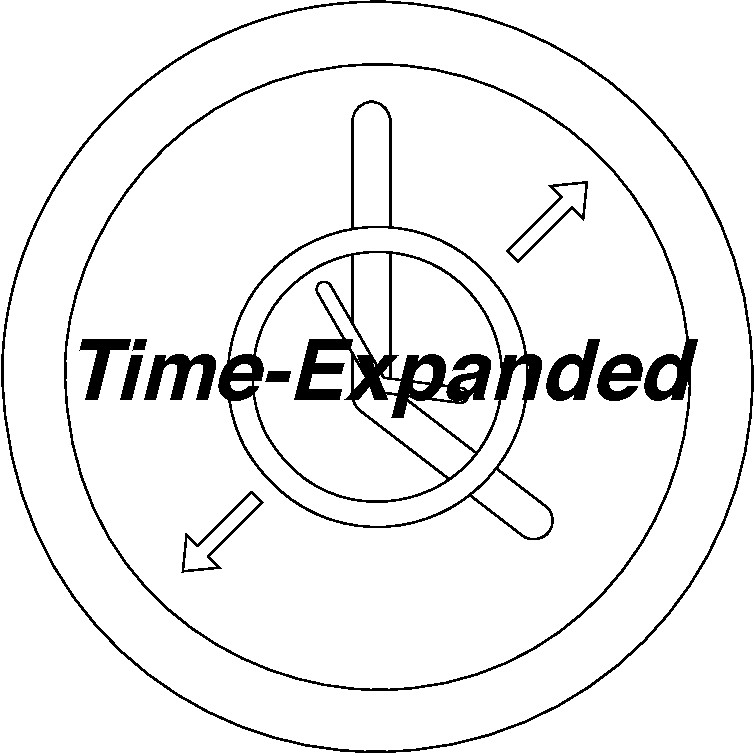
\includegraphics[width=.50\linewidth]{images/time-expanded/title.pdf} 
%	\end{center}
%\end{frame}


\begin{frame}{Das Time-Expanded Modell}
\framesubtitle{Train-Edges}
	\begin{itemize}{}
		\item Modelliere jedes "{}\textbf{Event}"{} innerhalb einer Station als eigenen Knoten. 
	\end{itemize}

	\begin{center}
		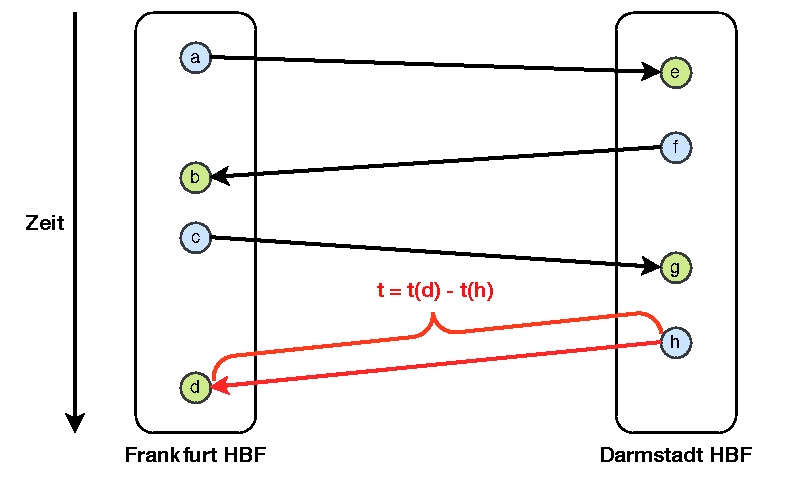
\includegraphics[width=.72\linewidth]{images/time-expanded-basic.pdf} 
	\end{center}
\end{frame}


\begin{frame}{Das Time-Expanded Modell}
\framesubtitle{Waiting-Edge}
	\begin{itemize}
		\item Erstelle eine Stationsinterne Kante, die \textbf{Exchange-Edge}. 
	\end{itemize}

	\begin{center}
	\hspace{5em}
		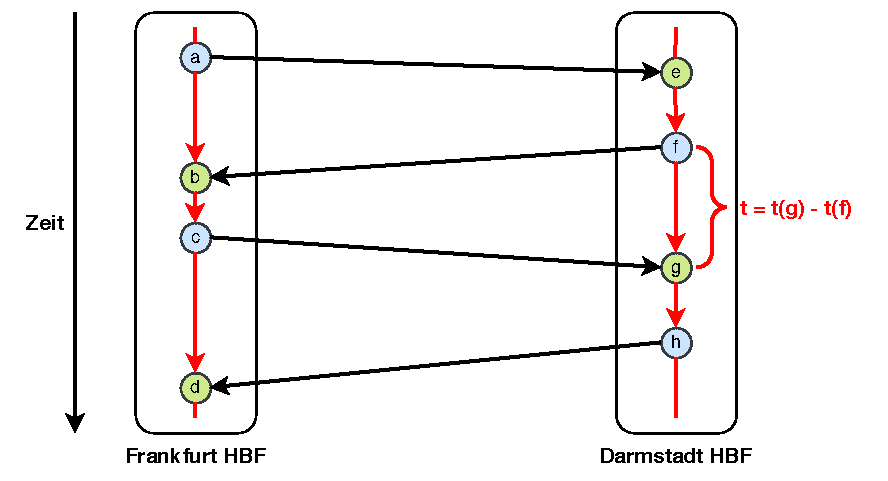
\includegraphics[width=.78\linewidth]{images/time-expanded-basic-2.pdf} 
	\end{center}
\end{frame}


%\begin{frame}{Das Time-Expanded Modell}
%\framesubtitle{Was bringt uns das Ganze jetzt?}
%\vspace{6em}
%\begin{center}
%	\begin{LARGE}
%		Kanten innerhalb einer Station $\approx$ "{}Umstiege"{}
%	\end{LARGE}
%\end{center}
%\end{frame}


\begin{image-frame}
\begin{frame}{}
	\vspace{-1em}
	\begin{center}
		\begin{tikzpicture}
			\node (img1) {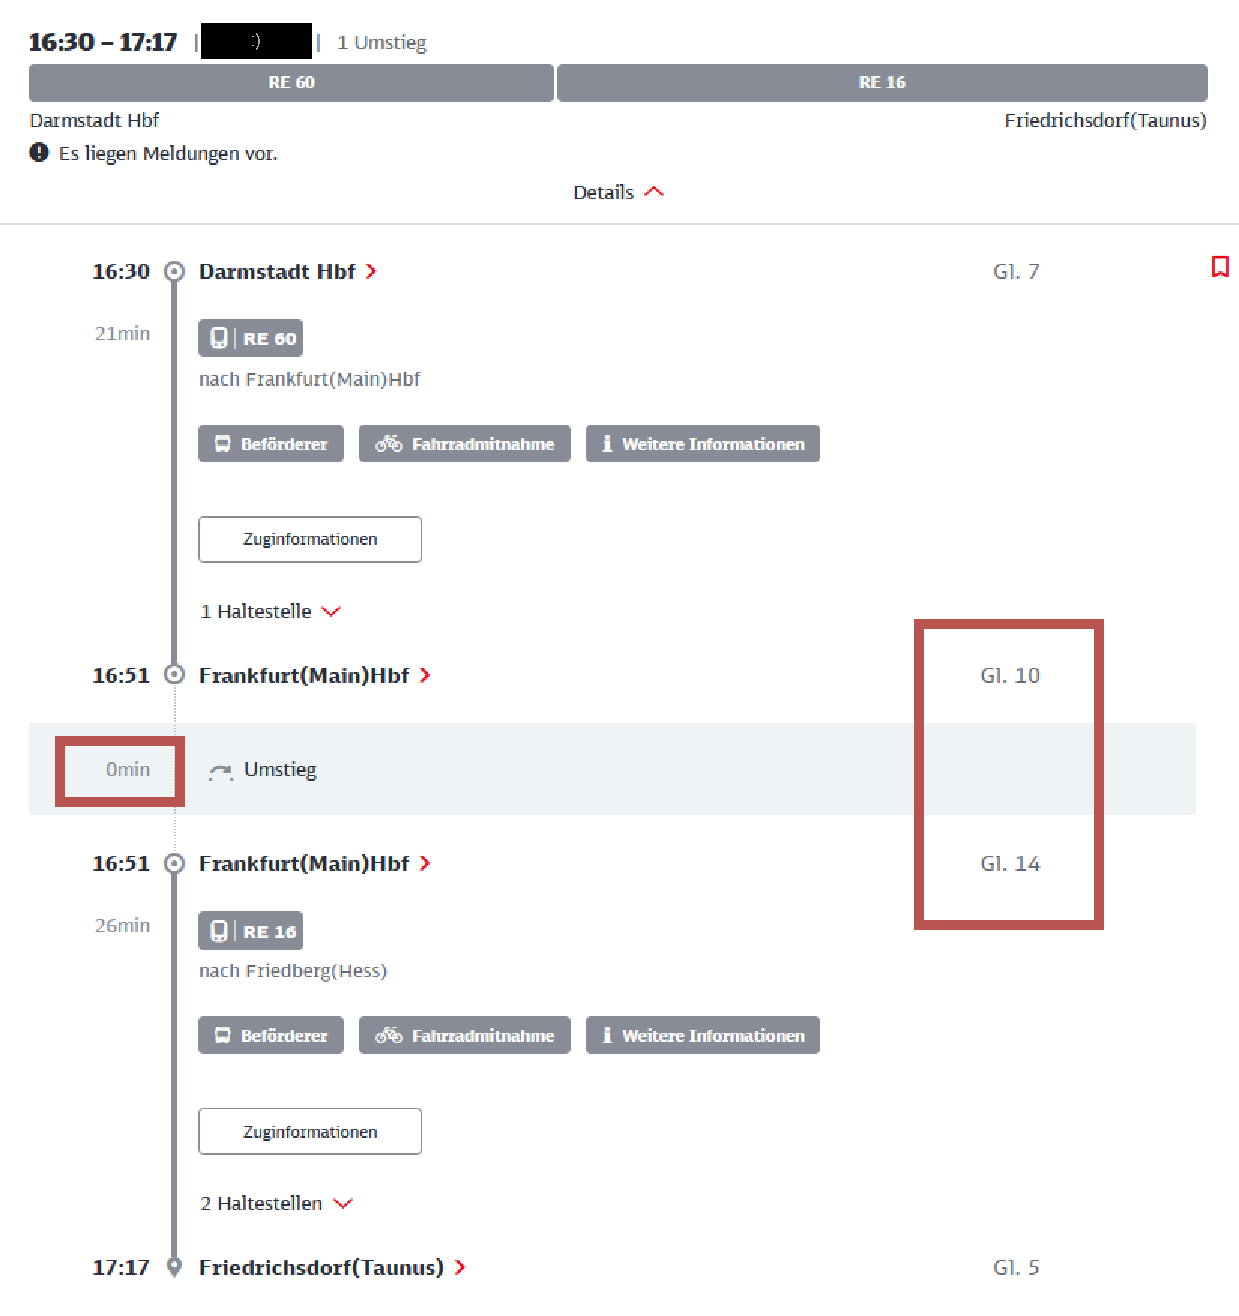
\includegraphics[width=.75\linewidth]{images/time-expanded_darmstadt-fdorf-no-interchange-time.pdf}};
			%\pause
			%\node (img2) at (img1.center) {
\includegraphics[height=3cm]{images/thinkingning.png}};
		\end{tikzpicture}
	\end{center}
\end{frame}
\end{image-frame}


\subsection{Umstiegszeiten}
\begin{frame}{Frage 3}
\begin{center}
	\vspace{6em}
	\begin{Large}
		Wie modelliere ich Umstiegszeiten mit "{}Puffer"{}?
	\end{Large}
\end{center}
\end{frame}


\begin{frame}{2. Griff in die Terminologie-Kiste}
	\framesubtitle{Realistische Umstiegsregeln}
	\begin{itemize}
		\item Definiere \textcolor{green}{Konstante} und \textcolor{red}{Variable} Umstiegsregeln:
		\begin{enumerate}
			\item \textcolor{green}{Standard-Umstiegszeit für alle Züge}
			\item \textcolor{red}{Regeln basierend auf Transferklassen \& Zuglinien}
			\item \textcolor{red}{Regeln zwischen einzelnen Zügen}
		\end{enumerate}
	\end{itemize}
\end{frame}


\begin{frame}{Konstante Umstiegszeiten}
	\begin{itemize}
		\item Spalte Exchange-Edge in Ankunfts- und Abfahrtsknoten
	\end{itemize}

	\begin{center}
		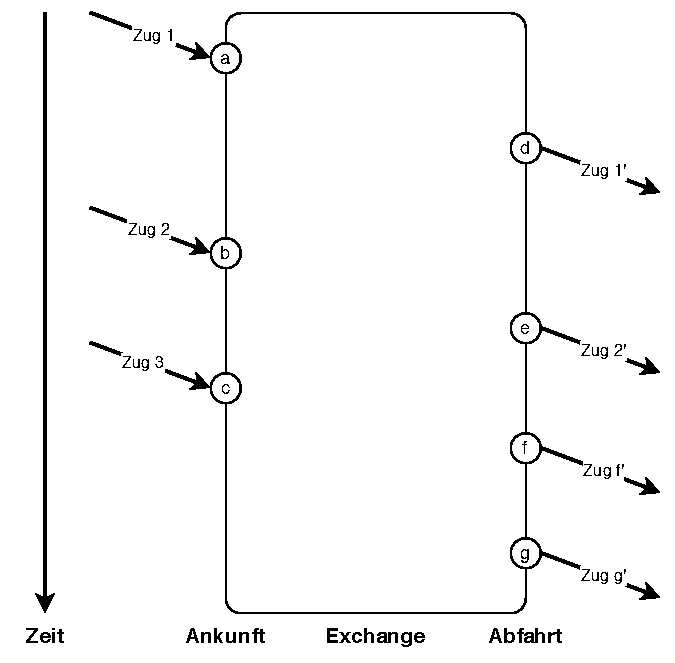
\includegraphics[height=5.8cm]{images/time_expanded_constant_interchange_0.pdf} 
	\end{center}
\end{frame}


\begin{frame}{Konstante Umstiegszeiten}
	\begin{itemize}
		\item Erstelle neue Exchange Edge
	\end{itemize}

	\begin{center}
		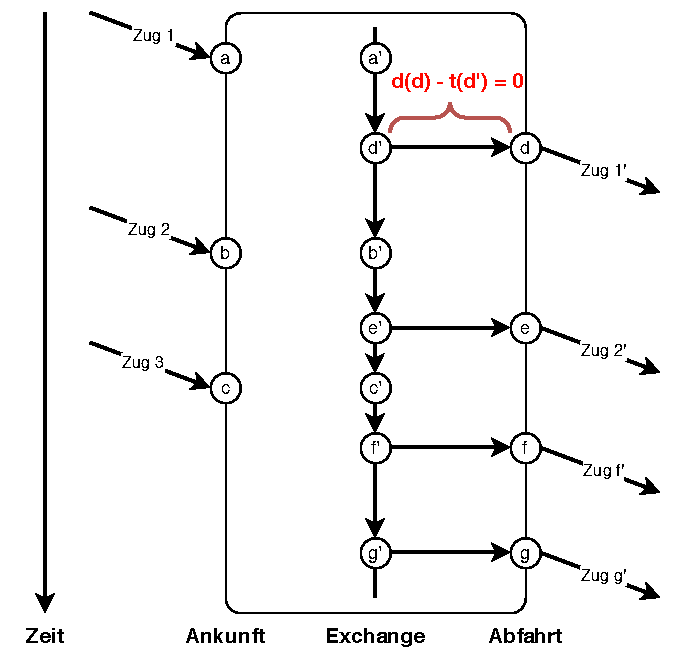
\includegraphics[height=5.8cm]{images/time_expanded_constant_interchange_1.pdf} 
	\end{center}
\end{frame}


\begin{frame}{Konstante Umstiegszeiten}
	\begin{itemize}
		\item Kanten von Ankunft $\rightarrow$ Exchange-Edge basierend auf min. Umstiegszeit
	\end{itemize}

	\begin{center}
		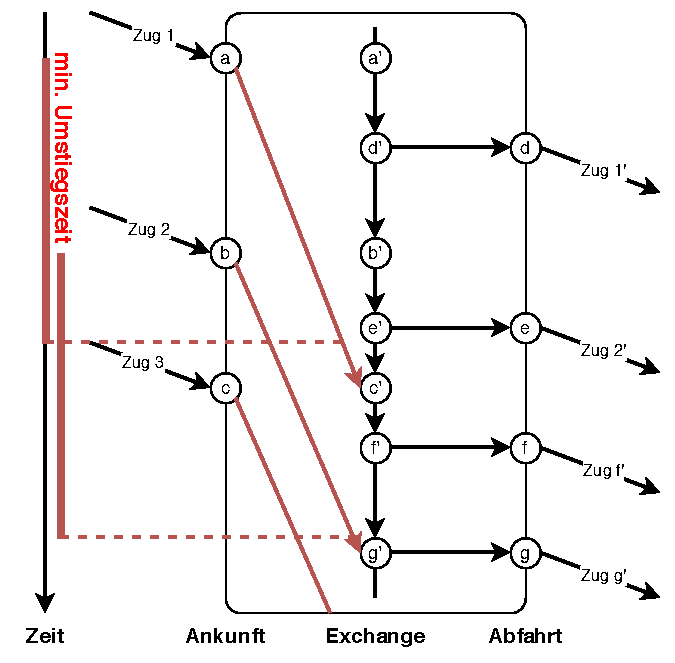
\includegraphics[height=5.8cm]{images/time_expanded_constant_interchange_2.pdf} 
	\end{center}
\end{frame}


\begin{frame}{Variable Umstiegszeiten}
	\begin{itemize}
		 \item Erstelle Kanten von Ankunft $\rightarrow$ Abfahrt des selben Zuges
	\end{itemize}

	\begin{center}
		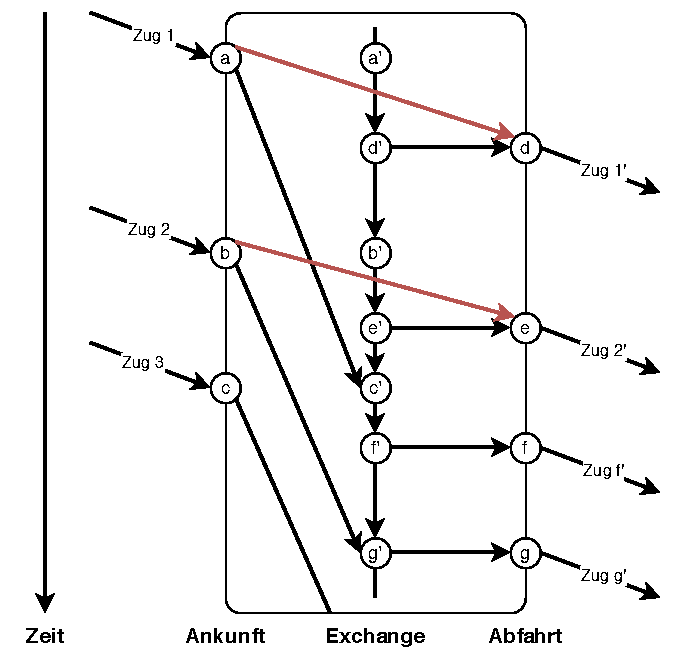
\includegraphics[height=5.8cm]{images/time_expanded_constant_interchange_3.pdf} 
	\end{center}
\end{frame}



\begin{frame}{Variable Umstiegszeiten}
	\begin{itemize}
		\item Weitere variable Umstiegszeiten als zzgl. Kanten
	\end{itemize}

	\begin{center}
		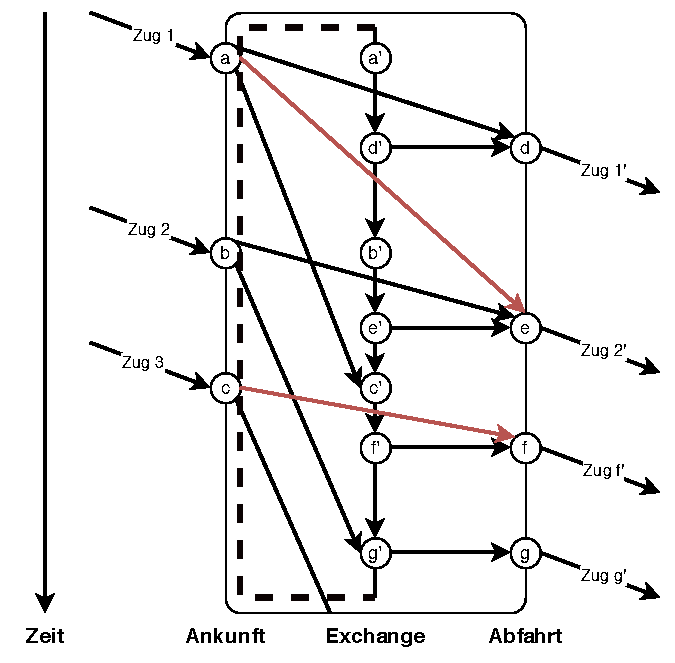
\includegraphics[height=5.8cm]{images/time_expanded_variable_interchange.pdf} 
	\end{center}
\end{frame}


\begin{frame}{Taktfahrplanmodellierung}
	\begin{itemize}
		\item Taktfahrplanmodellierung via Exchange-Edge-Schleife
	\end{itemize}

	\begin{center}
		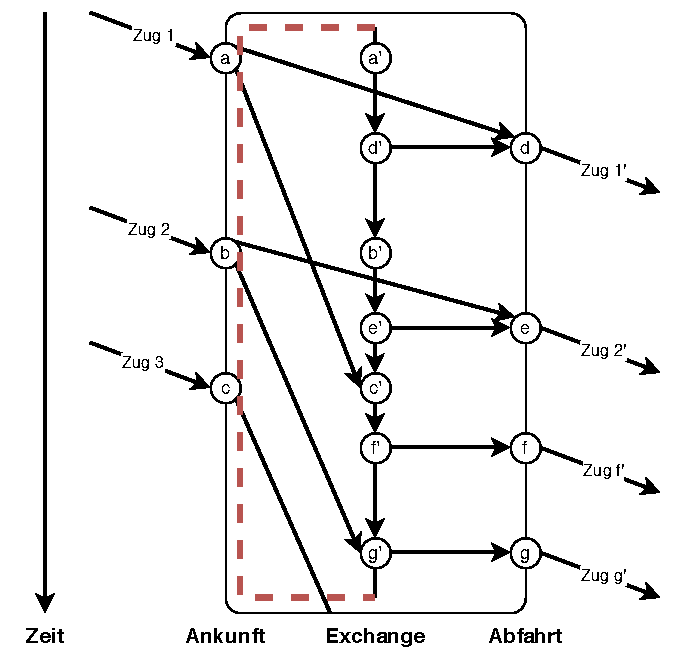
\includegraphics[height=5.8cm]{images/time_expanded_constant_interchange_4.pdf} 
	\end{center}
\end{frame}


\begin{frame}{Time-Expanded}
	\framesubtitle{Alle Konzepte auf einen Blick}
	\begin{center}
		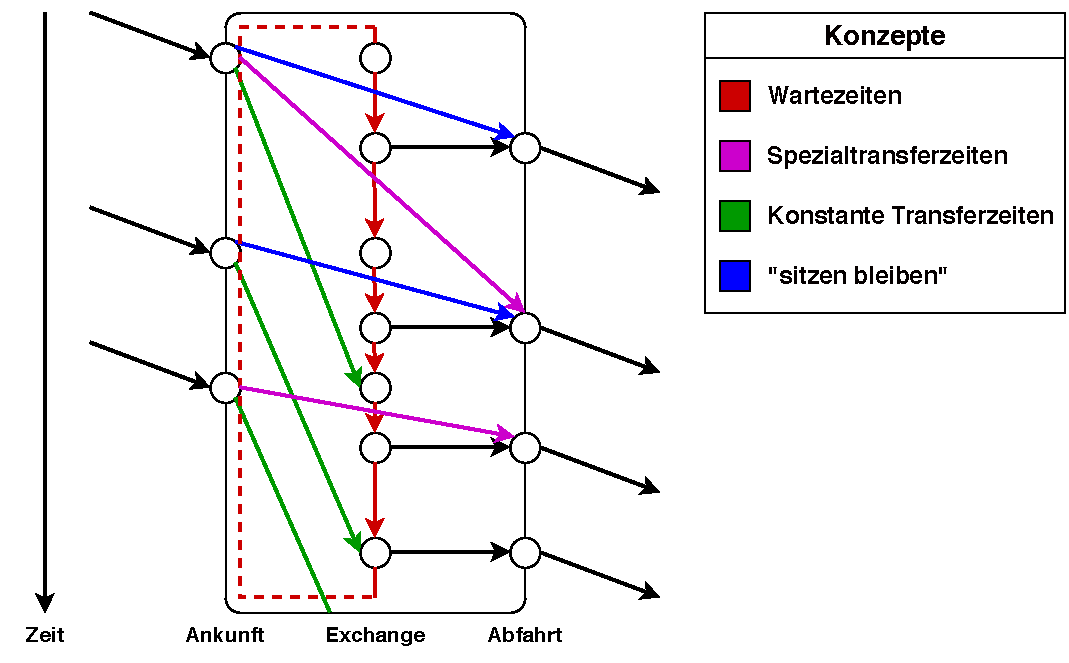
\includegraphics[height=6cm]{images/time-expanded/overview.pdf} 
	\end{center}
\end{frame}


\subsection{Verfeinerungen}
%\begin{frame}{Verfeinerung 1: Verkehrstage}
%	\begin{block}{Problem}
%		Der Takt unseres Fahrplans ist nicht nur ein Tag!
%	\end{block}
%
%	\begin{itemize}
%		\item Wie würde unser Graph wachsen, wenn wir $N$ Tage modellieren würden?
%		\begin{itemize}
%			\item Wir hätten etwa $N$-mal so viele Knoten und Kanten!
%		\end{itemize}
%	\end{itemize}
%
%\end{frame}


\begin{frame}{Verfeinerung 1: Verkehrstage}
	\begin{itemize}
		\item Versehe Knoten mit Zeit $t_{Absolut} \mod 1440$
		\begin{itemize}
			\item $t_{Absolut} \in [0, N \cdot 1440]$
		\end{itemize}
		\item Versehe Kanten mit einer Liste an Verkehstagen: $[d]$, $d \in N$
		\item Nutze Absolute Zeit beim SP-Durchlauf:
	\end{itemize}

	\begin{equation*}
		d_i = floor(\frac{t_{Anfrage}}{1440})
	\end{equation*}

	\begin{itemize}
		\item Und wenn der Zug an Tag $d_i$ fährt:
	\end{itemize}

	\begin{equation*}
		length(E) = (t_{Ankunft} - t_{Abfahrt}) \mod 1440
	\end{equation*}
\end{frame}


\begin{frame}{Verfeinerung 1: Verkehrstage}
\framesubtitle{Das ganze als Visuelles Beispiel}
	\begin{center}
		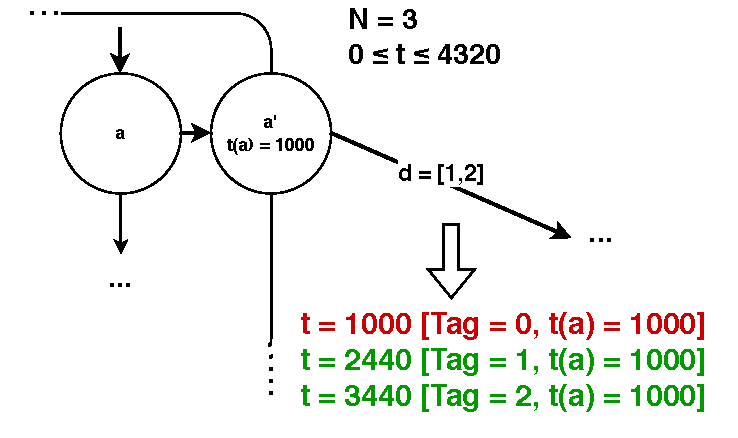
\includegraphics[height=6cm]{images/time-expanded/verkehrstage-beispiel.pdf} 
	\end{center}
\end{frame}


%\begin{frame}{Verfeinerung 1: Verkehrstage}
%	\begin{block}{Problem}
%		Wie behandeln wir besuchte Knoten beim SP-Durchlauf, die invalide sind?
%	\end{block}
%
%	\begin{itemize}
%		\item Als Beispiel am Dijkstra: 
%		\begin{itemize}
%			\item $dist \rightarrow \infty$
%			\item Füge Knoten wieder am Ende des Sets ein ("{}Nächster"{} Tag).
%		\end{itemize}
%	\end{itemize}
%	\vspace{7em}
%	Weitere Verfeinerungen sind möglich\footnote{(Pyrga et. al.: \textit{Efficient Models for Timetable Information in Public Transportation Systems})}...
%\end{frame}


\begin{frame}{Verfeinerung 2: Fußwege}
	\framesubtitle{Die Rückkehr der Terminologie-Kiste}
	\begin{block}{Frage}
		Was macht Fußwege so besonders?
	\end{block}
	\begin{itemize}
		\item Fußwege können zu jeder Zeit genutzt werden
		\item Man könnte sagen sie sind... \textit{Zeitabhängig} (Time-Dependent)...
	\end{itemize}

	\begin{center}
		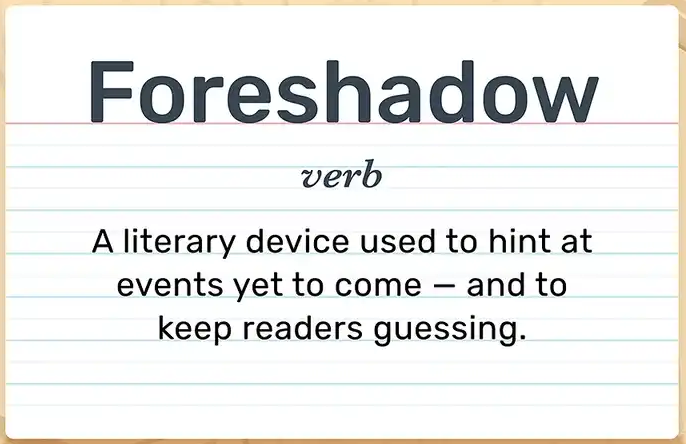
\includegraphics[height=4cm]{images/foreshadowing.png} 
	\end{center}
\end{frame}


\begin{frame}{Verfeinerung 2: Fußwege}
	\begin{itemize}
		\item Alle Fußwege im Graphen speichern ist nicht sinnvoll.
		% Beachte Fußwege nur, wenn wir eine arrival-node verlassen
		\item Speichere Wege in jeder Station, maskiere Wege in Suchanfragen als Kanten zwischen Stationen
		\begin{itemize}
			\item Durchsuche Fußwege, wenn eine Arrival-Node bearbeitet wird 
		\end{itemize}
		% Wenn wir N stationen im Umkreis haben, und Fußwege zu den Stationen < departure_interval sind, dann ist evtl. eine Verbindung mit Fußweg als erste "Kante" die beste!
		% Starte Dijkstra mit intialer zeit != 0, der Zeit des Fussweges
		\item Beachte Fußwege beim Start einer Reise!
	\end{itemize}
\end{frame}


\begin{frame}{Größenordnungen}
	\begin{itemize}
		\item Ein paar Zahlen im Jahr 2008 (\textbf{nur} Schienenpersonenvekehr):
	\end{itemize}
\vspace{3em}
	\begin{center}
		\begin{tabular}{ c|c } 
			Anzahl an Knoten & \\
 			\hline
 			Ankunft & 801.8 Tsd. \\
 			Abfahrt & 801.8 Tsd. \\
 			Change & 556.6 Tsd. \\
 			\hline
 			Gesamt & 2160.2 Tsd.
		\end{tabular}
	\end{center}
\end{frame}


\begin{frame}{Größenordnungen}
	\begin{itemize}
		\item Ein paar Zahlen im Jahr 2008 (\textbf{nur} Schienenpersonenvekehr):
	\end{itemize}
	\vspace{1em}
	\begin{center}
		\begin{tabular}{ c|c } 
			Anzahl an Kanten & \\
 			\hline
 			Zug & 801.8 Tsd. \\
 			Weiterfahrt & 733.7 Tsd. \\
 			\textit{Leaving} & 796.7 Tsd. \\
 			\textit{Entering} & 79\textit{6}.7 Tsd. \\
 			\textit{Waiting} & 556.6 Tsd. \\
 			Besondere Umstiege & 20.2 Tsd. \\
 			\hline
 			Gesamtanzahl & 3705.7 Tsd.
		\end{tabular}
	\end{center}
	\begin{block}{Erinnerung}
		68073 Zuglinien $\rightarrow 801.8k - 68k \approx 133k$
	\end{block}
\end{frame}



\section{Modell 2: Time-Dependent}
\begin{frame}
	\vspace{-3em}
	\begin{center}
		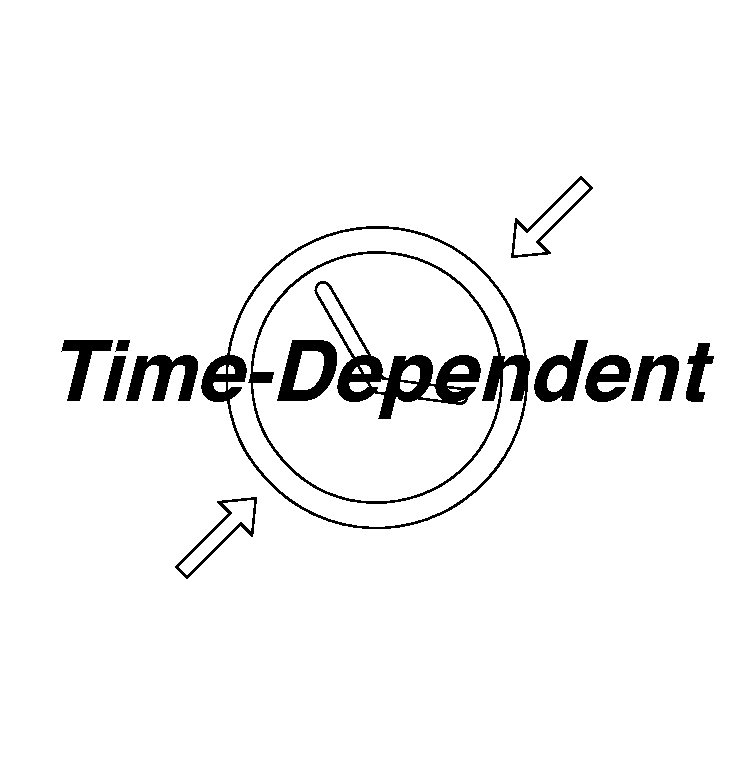
\includegraphics[width=.78\linewidth]{images/time-dependent/title.pdf} 
	\end{center}
\end{frame}


\begin{frame}{Das Time-Dependent Modell}
	\begin{itemize}
		\item Denken wir zurück an das erste Beispiel...
	\end{itemize}

	\begin{center}
		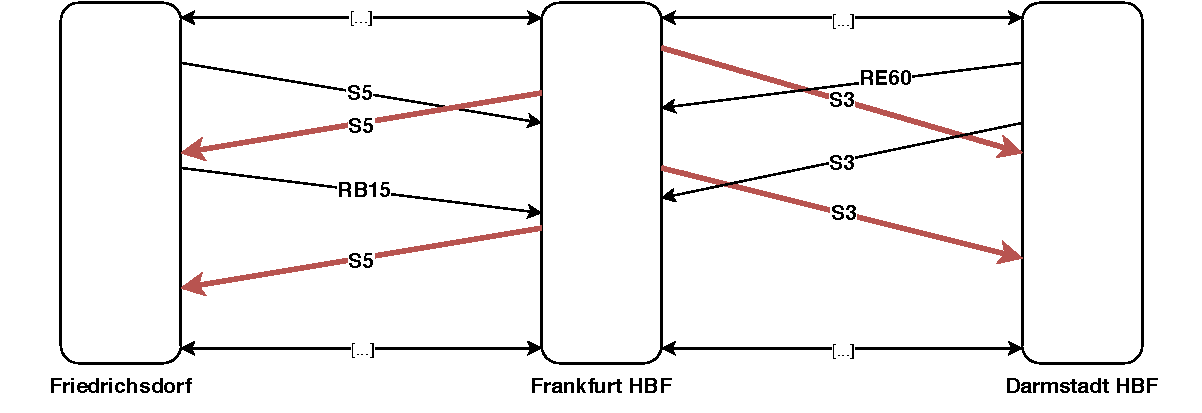
\includegraphics[width=\linewidth]{images/simple-approach-timed-3.pdf}
	\end{center}
\end{frame}


\begin{frame}{Das Time-Dependent Modell}
	\begin{itemize}
		\item Jetzt bauen wir das ganze etwas um...
	\end{itemize}

	\begin{center}
		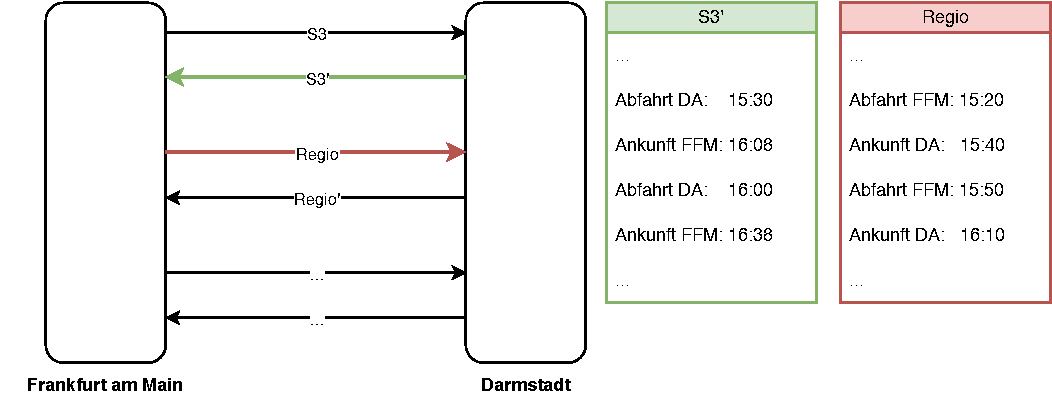
\includegraphics[width=\linewidth]{images/time-dependent/basic.pdf}
	\end{center}
\end{frame}

\begin{frame}{Das Time-Dependent Modell}
	\begin{itemize}
		\item Oder etwas formeller:
	\end{itemize}

	\begin{center}
		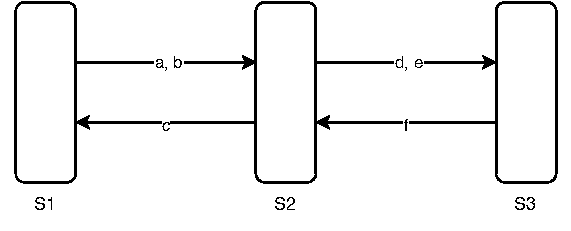
\includegraphics[width=\linewidth]{images/time-dependent/formal.pdf}
	\end{center}
\end{frame}


\begin{frame}{Das Time-Dependent Modell}
	\begin{itemize}
		\item Wir definieren für jede Kante $(u,v)$ eine\* Funktion $f(t): \mathcal{T} \rightarrow \mathcal{T}$.
		\begin{itemize}
			\item $t \in \mathcal{T}$, $\mathcal{T} \triangleq$ Zeit.
		\end{itemize}
	\end{itemize}
	\vspace{2em}
	\pause
	\begin{itemize}
		\item Dann ist unser Kantengewicht (\textit{Reisezeit}):
	\end{itemize}
	
	\begin{equation*}
		travel\_time(t) = f_{(u,v)}(t) - t
	\end{equation*}

	\vspace{4em}
	% z.B. Binärsuche auf geordneter Liste assoziiert mit {a, b} an Abfahrtszeiten von a
	\begin{block}{Frage}
		Wie sieht so eine Funktion in der Realität aus?
	\end{block}
\end{frame}

\subsection{Umstiegszeiten}
\begin{frame}{Das Time-Dependent Modell}
	\framesubtitle{Konstante Umstiegszeiten}
	\begin{itemize}
		\item Für konstante Umstiegszeiten definieren wir Zugrouten:
		\begin{itemize}
			\item Sei R eine Zugroute $S_0,S_1,...,S_{k - 1}, S_k$ für $k > 0$
			\pause
			\item Erlaubt: $S_i = S_j$, $i,j \in k$, für $i \neq j$ (Schleifen)!
		\end{itemize}
	\end{itemize}
	
	\begin{center}
		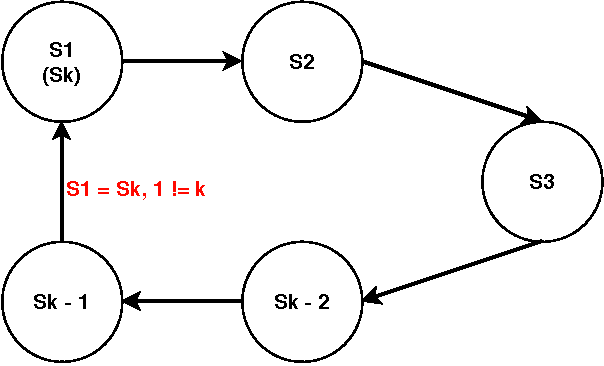
\includegraphics[height=12em]{images/time-dependent/zugroute.pdf}
	\end{center}
\end{frame}


\begin{frame}{Das Time-Dependent Modell}
	\framesubtitle{Konstante Umstiegszeiten}
	\begin{itemize}
		\item Jetze gruppieren wir alle Züge, die die gleiche Strecke fahren, in eine Zugroute
		\item \textbf{Was ist hier das Problem?}
	\end{itemize}
	
	\begin{center}
		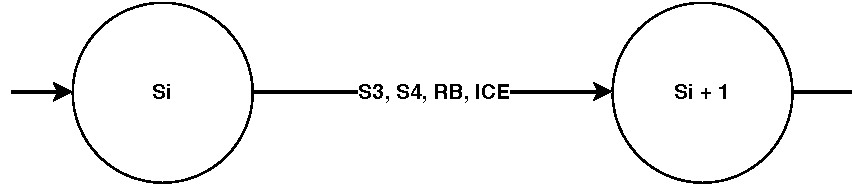
\includegraphics[width=\linewidth]{images/time-dependent/zugroute-problem.pdf}
	\end{center}
\end{frame}


\begin{frame}{Das Time-Dependent Modell}
	\framesubtitle{Konstante Umstiegszeiten}

	\begin{center}
		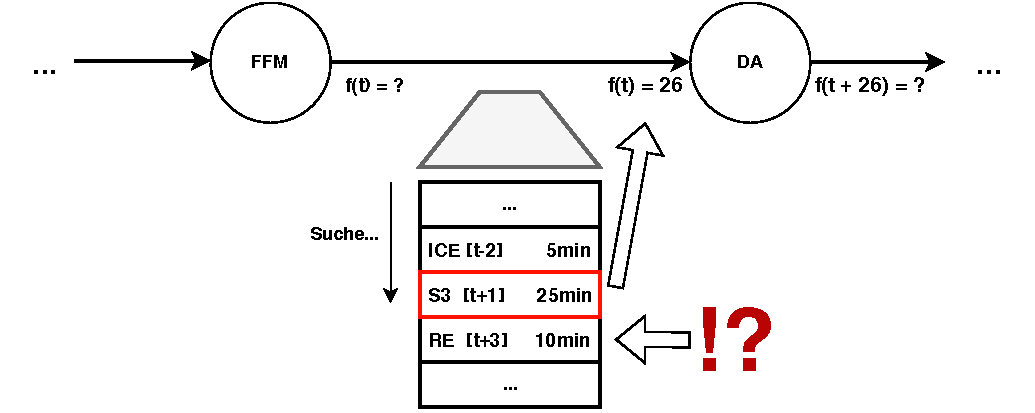
\includegraphics[width=\linewidth]{images/time-dependent/zugroute-problem-beispiel.pdf}
	\end{center}

	\pause
	\begin{block}{}
		In welchen Fällen aber wäre es doch besser, die S3 zu nehmen?
	\end{block}
\end{frame}


\begin{frame}{Das Time-Dependent Modell}
	\framesubtitle{Konstante Umstiegszeiten}
	\begin{itemize}
		\item Keine Züge $z_1,z_2$ dürfen $S_i$ um $t_1,t_2$ ($t_1 \leq t_2$) verlassen, und $z_2$ vor $z_1$ $S_{i + 1}$ erreichen!
		\item In diesem Fall spalten wir in einzelne Routen:
	\end{itemize}
	
	\begin{center}
		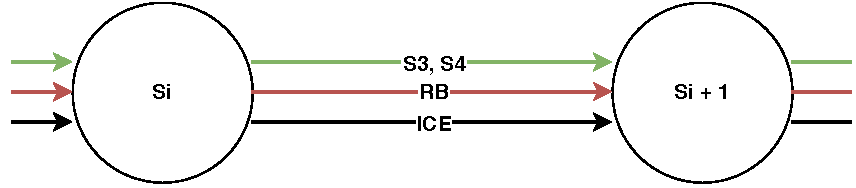
\includegraphics[width=\linewidth]{images/time-dependent/zugroute-loesung.pdf}
	\end{center}
\end{frame}


\begin{frame}{Das Time-Dependent Modell}
	\framesubtitle{Konstante Umstiegszeiten}
	\begin{itemize}
		\item Wir teilen eine Station in einen Stationsknoten $S$ und Routenknoten $r_i$
	\end{itemize}
	
	\begin{center}
		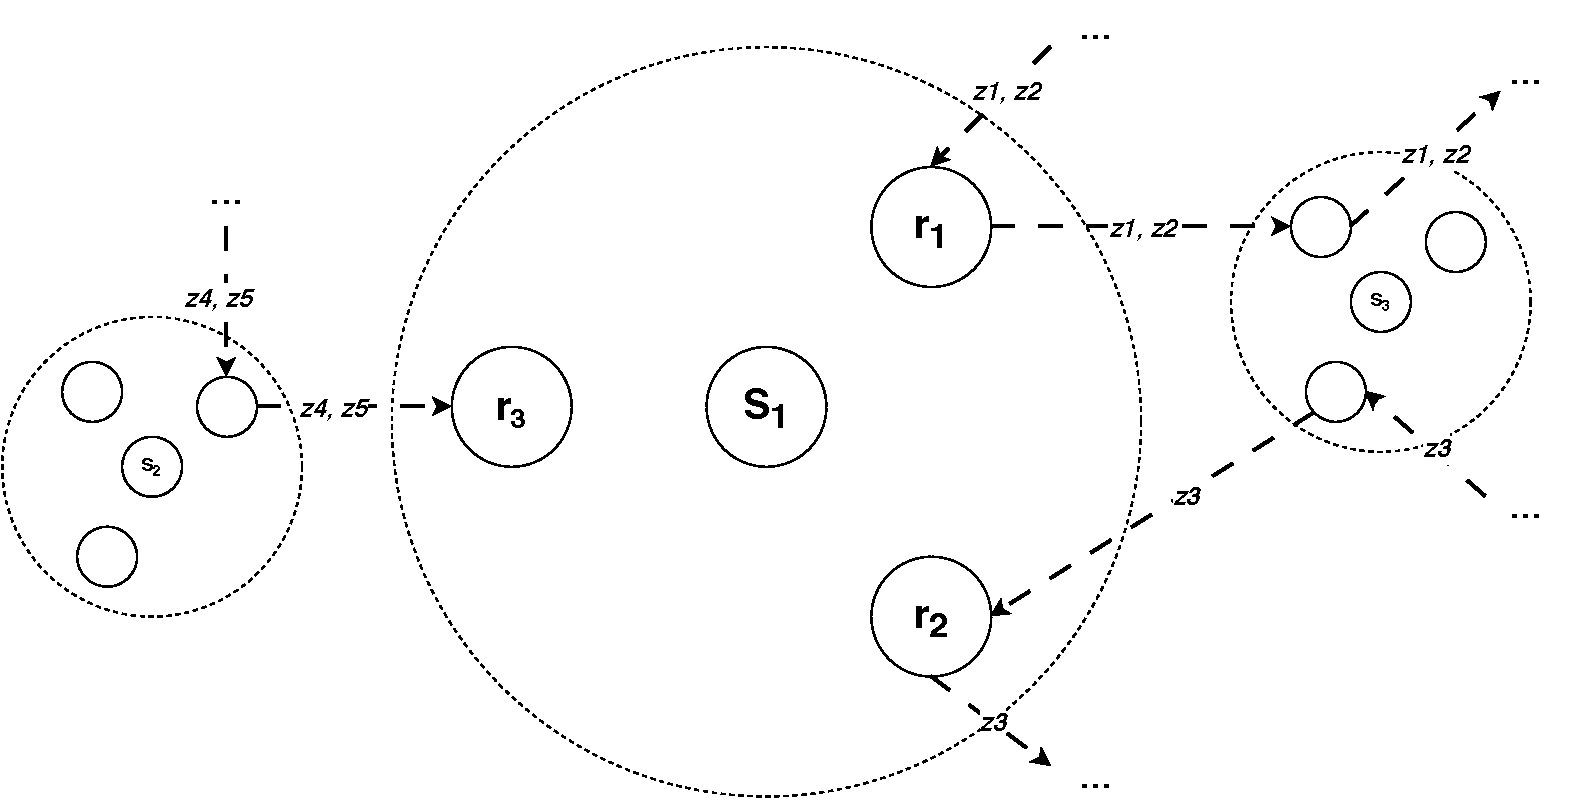
\includegraphics[width=.90\linewidth]{images/time-dependent/model_0.pdf}
	\end{center}
\end{frame}


\begin{frame}{Das Time-Dependent Modell}
	\framesubtitle{Konstante Umstiegszeiten}
	\begin{itemize}
		\item Wir erstellen Transferkanten mit \textit{ausgehenden} Transferkosten
	\end{itemize}

	% Ausgehende Kosten, optimierung, da die r-knoten den gleichen labelwert haben wie s
	% Daher können wir sie erstmal ignorieren (minimale prio) bzw erstmal komplett weglassen
	% dann später wieder einfügen
	\begin{center}
		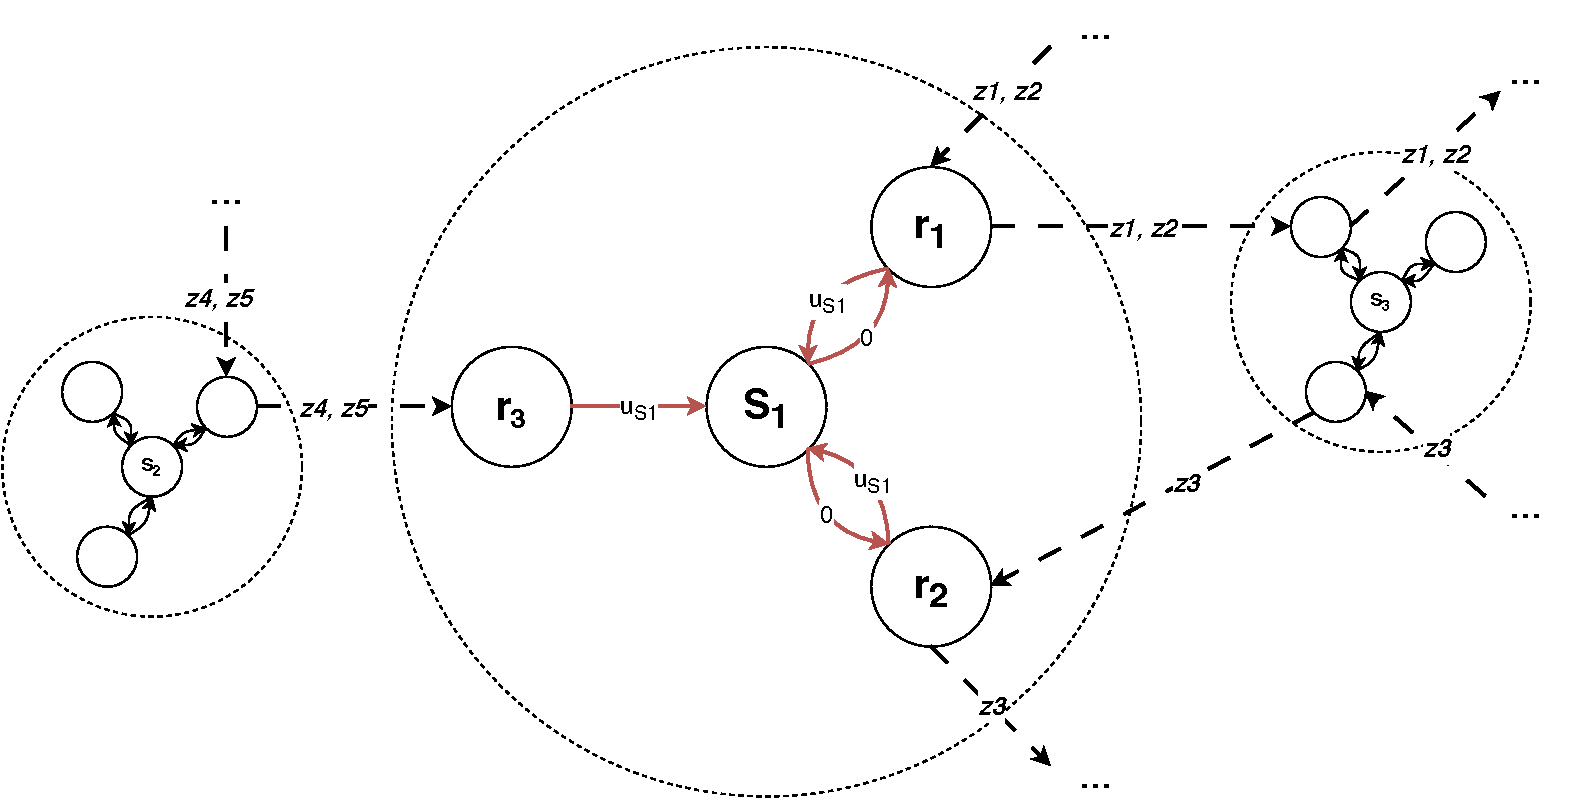
\includegraphics[width=.90\linewidth]{images/time-dependent/model_1.pdf}
	\end{center}
\end{frame}


\begin{frame}{Das Time-Dependent Modell}
	\framesubtitle{Variable Umstiegszeiten}
	\begin{itemize}
		\item Wir erstellen spezielle Kanten und Regeln zwischen Knoten
	\end{itemize}

	\begin{center}
		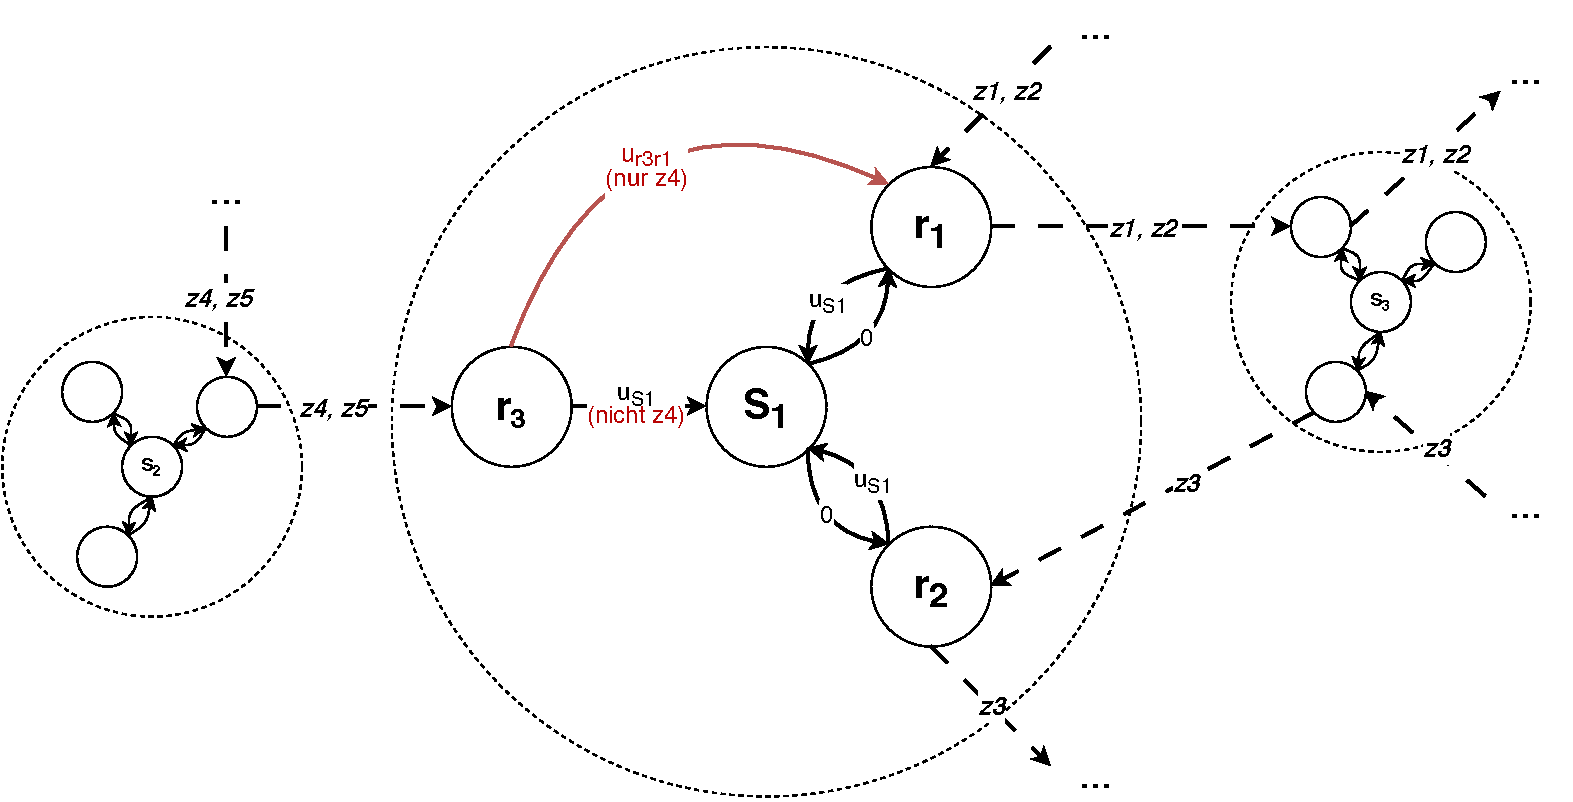
\includegraphics[width=.90\linewidth]{images/time-dependent/model_2.pdf}
	\end{center}
\end{frame}

\subsection{Verfeinerungen}
\begin{frame}{Fußwege}
	\begin{itemize}
		\item Fußwege sind immer abhängig von der Zeit, also einfach zu modellieren
	\end{itemize}

	\begin{center}
		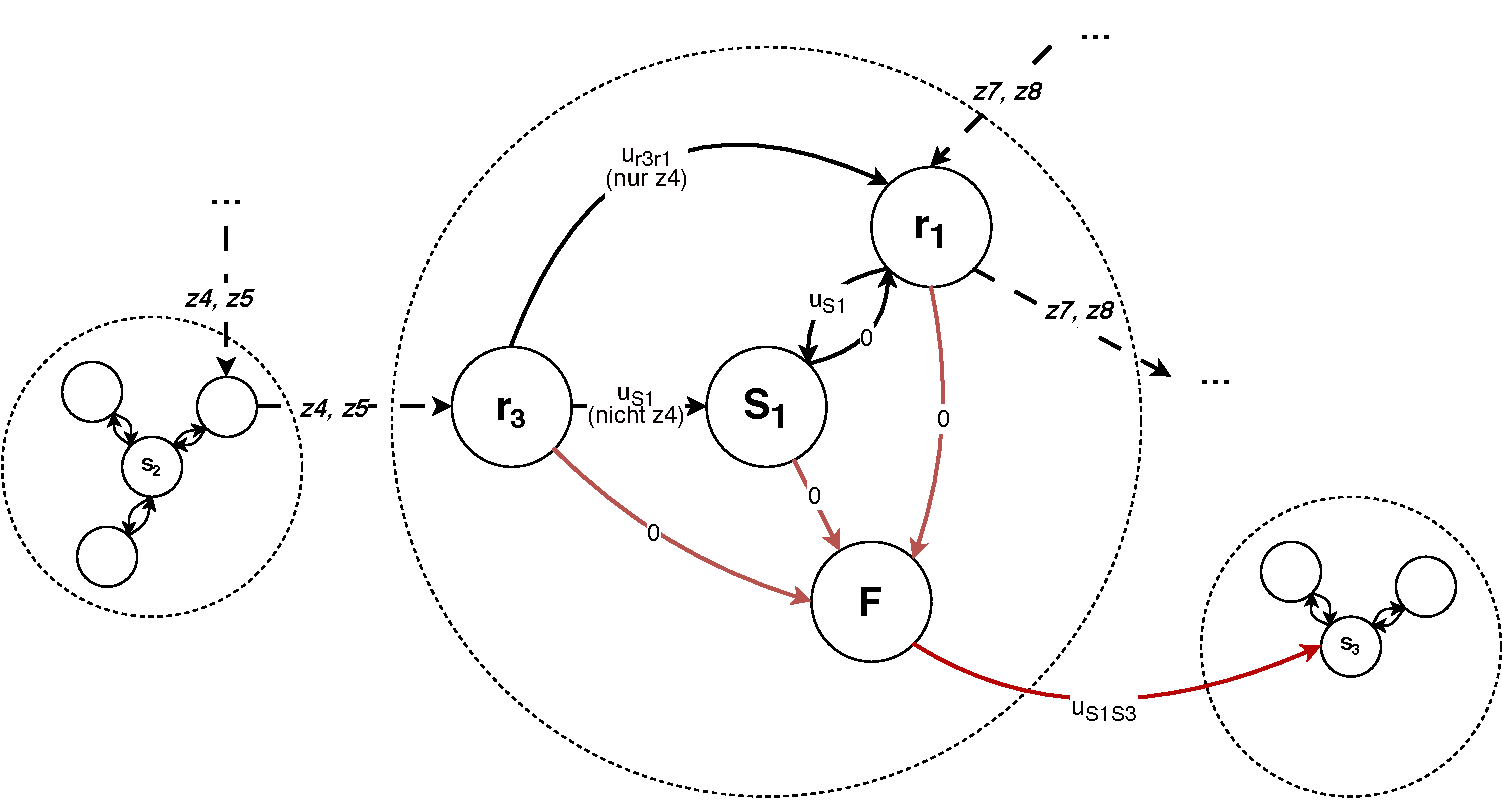
\includegraphics[width=.90\linewidth]{images/time-dependent/model_3.pdf}
	\end{center}
\end{frame}



















\section{Vergleiche}
\begin{frame}{Größenordnungen}
	\begin{itemize}
		\item DB Fahrplan 1996/97 (\textbf{nur} Schienenpersonenvekehr)\blfootnote{(Pyrga et al. \textit{Time-Expanded vs Time-Dependent Models for Timetable Information})}:
	\end{itemize}
	
	\begin{center}
		\begin{tabular}{ c|r|r } 
			& Time Expanded & Time Dependent \\
 			\hline
 			\hline
 			Knoten & 931746 & 6961 \\
 			Kanten & 1397619 & 18664 \\
 			\hline
		\end{tabular}
	\end{center}
	
	\vspace{2em}	
	
	\begin{center}
		\begin{tabular}{ l|c|c } 
			& Time Expanded & Time Dependent \\
 			\hline
 			\hline
 			Algorithmus & Dijkstra & Dijkstra + Binärsuche \\
 			$\varnothing{}$ Laufzeit & 44.17ms & 5.61ms \\
 			Besuchte Knoten & 33653 & 1515 \\
 			\hline
		\end{tabular}
	\end{center}

	$\rightarrow$ Mehr dazu im nächsten Vortrag!
\end{frame}


\begin{frame}{Performanz}
	\begin{itemize}
		\item Aber: Komplexität von TD wächst schnell mit mehr Kriteria und Regeln\blfootnote{(Pyrga et al.: \textit{Experimental Comparison of Shortest Path Approaches for Timetable Information}, 2004)}
		\item Also in realistischen Szenarien!
		\begin{itemize}
			\item TD nur $58\%$ schneller (in CPU-Zeit) als TE
		\end{itemize}
	\end{itemize}

\end{frame}



\section{Exkurs: Implementation in MOTIS}
\begin{frame}{Implementation in MOTIS}
	\framesubtitle{Graphenmodell}
	\begin{itemize}
		\item Time-Expanded mit Verfeinerungen
		\begin{itemize}
			\item Konstante und Variable Umstiegszeiten
			\item Verkehrstage
			\item Fußwege
		\end{itemize}
	\end{itemize}
\end{frame}

\begin{frame}{Implementation in MOTIS}
	\framesubtitle{Kantengewichtungen}

	\begin{itemize}
		\item Reisezeit ($t_{Ankunft} - t_{Abfahrt} \mod 1440$)
		\item Anzahl der Umstiege (Ankunfts- und Spezialkanten)
		\item Ticketpreise $\rightarrow$ Vortrag Spezialangebote
	\end{itemize}
\end{frame}


\begin{frame}{Implementation in MOTIS}
	\framesubtitle{Algorithmus}

	\begin{itemize}
		\item Viele Algorithmusverfeinerungen und Spezialattribute
		\begin{itemize}
			\item Thema des nächsten Vortrags!
		\end{itemize}
	\end{itemize}
\end{frame}

%\begin{frame}{Das dritte Graphenmodell}
%	\framesubtitle{Es ist das dritte Graphenmodell mit einem Klappstuhl?!?!!}
%	
%	\begin{itemize}
%		\item In MOTIS gibt es noch ein drittes großes Graphenmodell: Den %\textbf{Abhängigkeitsgraphen}
%		\item Abhängigkeiten zwischen Zügen und Stationen
%		\item Wichtig für \textbf{Verspätungen}!
%	\end{itemize}

%	\begin{center}
%		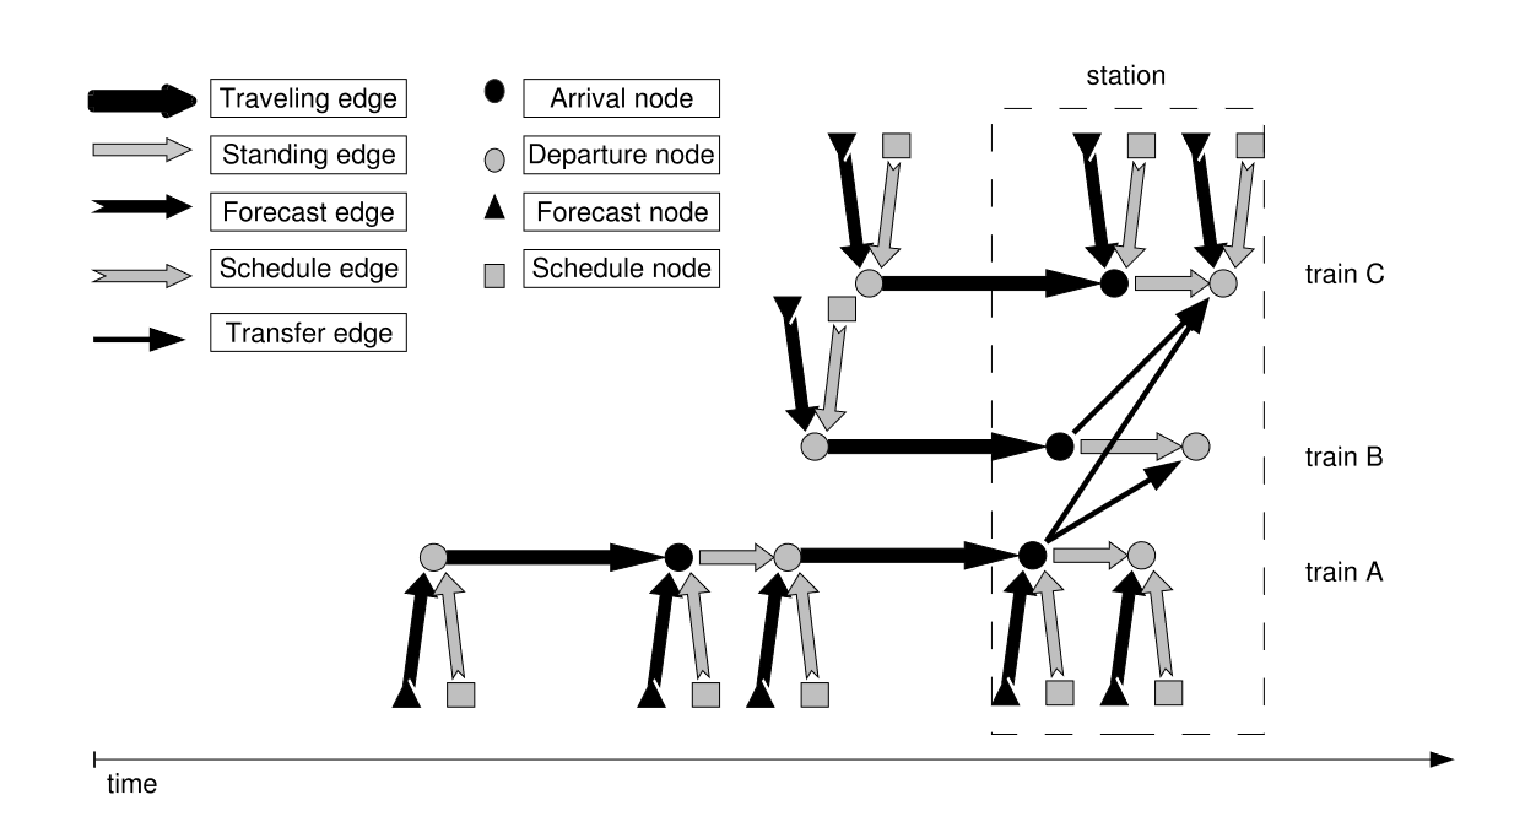
\includegraphics[height=4cm]{images/dependency/dependency-graph.pdf} 
%	\end{center}
%\end{frame}


\begin{frame}{Zusammenfassung}
	\framesubtitle{Sachen zum Mitnehmen für die späteren Vorträge...}
	\begin{itemize}
		\item Time-Expanded vs. Time-Dependent
		\begin{itemize}
			\item Umstiegszeiten, Fußwege, Takt
			\item In MOTIS: Time-Expanded
		\end{itemize}
		\item Größenordnungen der Graphen unterscheiden sich stark
		\item Für realistische Anwendung: Jeweils unterschiedliche Verfeinerungen und Anpassungen notwendig
	\end{itemize}

\end{frame}

%\begin{frame}{Time-Expanded}
%	\framesubtitle{Nochmal zum Mitnehmen}
%	\begin{center}
%		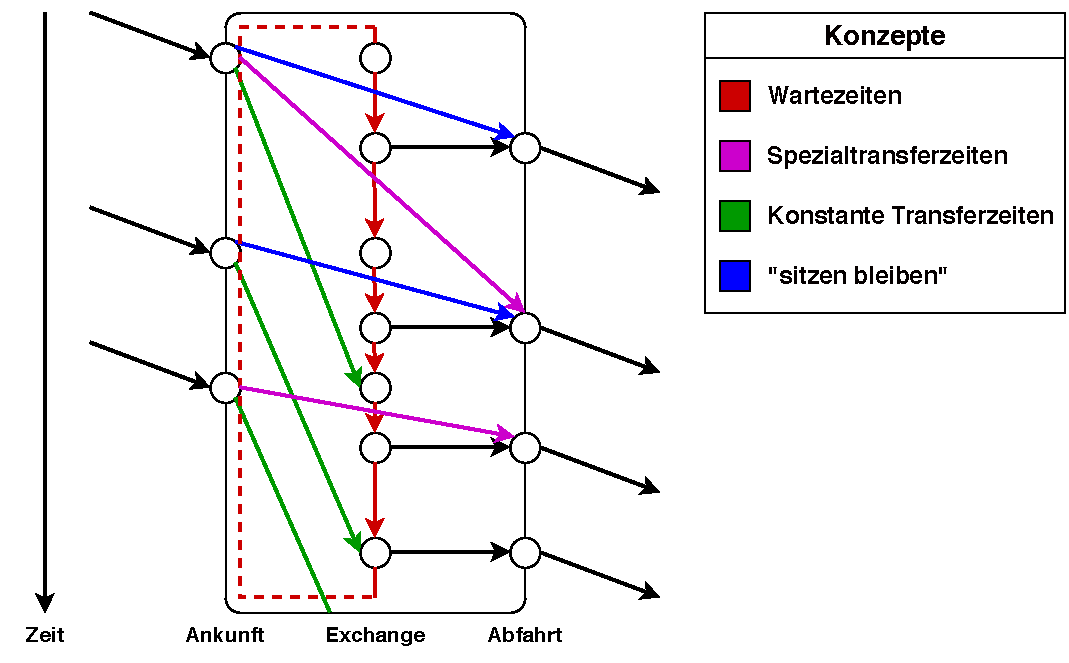
\includegraphics[height=6cm]{images/time-expanded/overview.pdf} 
%	\end{center}
%\end{frame}


\begin{frame}{Literaturquellen}
	\begin{itemize}
		\item Schnee, Matthias, \textit{Fully Realistic Multi-Criteria Timetable Information Systems}, 2009, Technische Universität Darmstadt
		\item Evangelia Pyrga, Frank Schulz, Dorothea Wagner, Christos Zaroliagis, \textit{Towards Realistic Modeling of Time-Table Information through the Time-Dependent Approach}, Electronic Notes in Theoretical Computer Science, Volume 92, 2004, Pages 85-103
		\item Evangelia Pyrga, Frank Schulz, Dorothea Wagner, Christos Zaroliagis \textit{Efficient models for timetable information in public transportation systems.} ACM Journal of Experimental Algorithmics, Volume 12, 2007
		\item Evangelia Pyrga, Frank Schulz, Dorothea Wagner, Christos Zaroliagis  \textit{Two Approaches for Time-Table Information: a Comparison of Models and Performance.}, Konstanzer Schriften in Mathematik und Informatik, Volume 190, 2003
\end{itemize}
\end{frame}


\begin{frame}{Weitere Bildquellen nach Folie}
	\begin{itemize}
		\item Verkehrsmittel (8): Wikimedia
		\item Portrait von Edsger W. Dijkstra (3, 4): https://de.wikipedia.org/wiki/Edsger\_W.\_Dijkstra (06.01.23)
		\item Fahrplanauszüge (3, 4, 18, 19): www.rmv.de und www.bahn.de (07.01.23)
		\item Abhängigkeitsgraph (55), (sowie \textit{alle weiteren Diagramme in Eigenanfertigung nach}) Schnee, Matthias, \textit{Fully Realistic Multi-Criteria Timetable Information Systems}, 2009, Technische Universität Darmstadt
	\end{itemize}
\end{frame}


\end{document}

